\documentclass[]{uc2pfecaneva}



\begin{document}
    \setlength{\parskip}{6pt}
    \tableofcontents
    \setcounter{chapter}{2}
    \chapter{Developement}\label{ch:developement}
    \newpage

    \section{Introduction}\label{sec:introduction}

    Having discussed the conception phase of our application in the last chapter, the next part of this report will focus on application implementation, which will be the last part. \\
    Implementation is the process of bringing together the entire design process, in which we ensure that the system is ready for end-user use. \\
    We first present our choice of the working environment, where we specify the hardware and software environment that we used to create our application, after that, we presented the programming languages and frameworks that we used and the motivation for using them, right after that we discussed the security aspect for our choices and the techniques we adopted to secure our system, then we present some interfaces created to illustrate the operation of some system activities, finally we finished with a conclusion summarizing this chapter.

    \section{System architecture}\label{sec:system-architecture}

    In order to boost our system efficiency we divided it to three separate parts that we gonna call "Projects" that communicate with each other in a specific way, each team member was responsible for a project yet contributes in the other projects.

    \begin{figure}[h]
        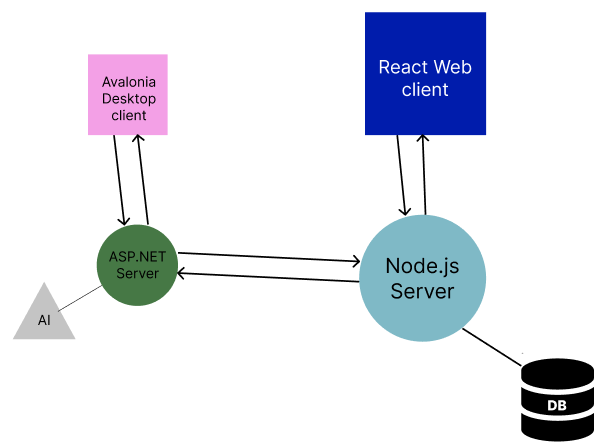
\includegraphics[width=250pt]{images/SystemArch}
        \centering
        \caption{System architecture visualisation}
        \label{fig:figure}
    \end{figure}


    The first project is the Web client application, was built using ReactJs, it’s the main client app we have, used for mostly for everything. \\
    The second project is the Main server api, was built using NodeJs, it’s the only project that can talk to the Database, it also handles all requests from the web client app. \\
    The last project of the system was made for the Student to take exams on, we chose not to make students take exams on the main web application that runs on the browser for these reasons:

    \begin{itemize}
        \item You can’t prevent the student from recording the browser and share it.
        \item You can’t monitor the student activity and the programs opened in the background.
        \item You can’t kill or close programs that might be used for cheating.
        \item You can’t tell if the student has an external monitor that he might be used for cheating.
    \end{itemize}


    These problems lead us to chose to build a desktop client application using Avalonia, with it’s own separate server that’s dedicated only to handle requests coming from the desktop application, that was built using ASP.NET, the motivation to have an additional server was :

    \begin{itemize}
        \item Prevent the whole system from cracking down if one of the servers is down or hacked.
        \item Give the student the best performance and the shortest response time even when the main server is falling behind.
        \item The need of another server that can handle heavy calculations related to artificial intelligent.
        \item Allow the student to finish the exam and submit his answers even when the main server is down, the answers  will be stored in the secondary server until the main one is up again.
    \end{itemize}




    \section{Tools}
    In this section we will list all the tools that we used in our project and the motivation for using them. \\

    \noindent
    \begin{wrapfigure}{r}{0.10\textwidth}
        
\includegraphics[width=0.10\textwidth]{images/trello}
    \end{wrapfigure}
    \textbf{Trello: } A collaboration tool that organizes your projects into boards, We used it to track our progress on each chapter and assign tasks to members. 
    \clearpage
    \begin{wrapfigure}{R}{0.10\textwidth}
        
\includegraphics[width=0.10\textwidth]{images/github}
        \vspace{-30pt}
    \end{wrapfigure} \noindent
    \textbf{Github: } A code-hosting platform for version control and collaboration, We used it to host all of our project, including the thesis LaTeX files and PlantUML diagrams.
    each project in a separate repository, we also used Github actions to automate our builds with continuous integration.

    \begin{wrapfigure}{R}{0.10\textwidth}
        
\includegraphics[width=0.10\textwidth]{images/discord}
        \vspace{-30pt}
    \end{wrapfigure} \noindent
    \textbf{Discord: } A messaging social platform that gives you the ability to communicate using communities called “servers”, we created a small server for our project and used it as our main communication tool, we also used it to share resources and anything useful for our project, meetings between members were all organized and archived in discord.

    \begin{wrapfigure}{R}{0.10\textwidth}
        
\includegraphics[width=0.10\textwidth]{images/vscode}
        \vspace{-40pt}
    \end{wrapfigure} \noindent
    \textbf{Visual Studio Code: } A very known lightweight open-source cross-platform code editor by Microsoft.
    powered with it's large number of extensions and supporting community. \\
    Used to develop the ReactJs web application.

    

    \begin{wrapfigure}{R}{0.10\textwidth}
        
\includegraphics[width=0.10\textwidth]{images/vs}
    \end{wrapfigure} \noindent
    \textbf{Visual Studio 2022: } A cross-platform integrated development environment (IDE) developed by Microsoft, it’s used to develop computer programs, as well as websites, web apps, web services and mobile apps, we used Visual Studio to develop the Desktop client.
    we chose it because it has better support for Xaml and has a better Xaml designer.

    \begin{wrapfigure}{R}{0.10\textwidth}
        
\includegraphics[width=0.10\textwidth]{images/rider}
        \vspace{-30pt}
    \end{wrapfigure} \noindent
    \textbf{Jetbrains Rider: }  An IDE made by Jetbrains to develop .NET applications very similarly to Visual Studio but it has more features because it’s a paid product.
    We used Rider to develop the Web API for the Desktop client.
    We chose Rider because it’s more performant and has better code refactoring features.

    \begin{wrapfigure}{R}{0.10\textwidth}
        
\includegraphics[width=0.10\textwidth]{images/vm}
    \end{wrapfigure} \noindent
    \textbf{VMware Workstation}: VMware Workstation is a software solution that allows you to run multiple operating systems (including Windows virtual machines) on a single Windows or Linux computer, this allowed us to simulate a real-world application deployment environment (with each subsystem running in a separate virtual machine), which helped us solve more problems during the development phase and test the real settings as our system is being used by the final customers.  \\


    \begin{wrapfigure}{R}{0.10\textwidth}
        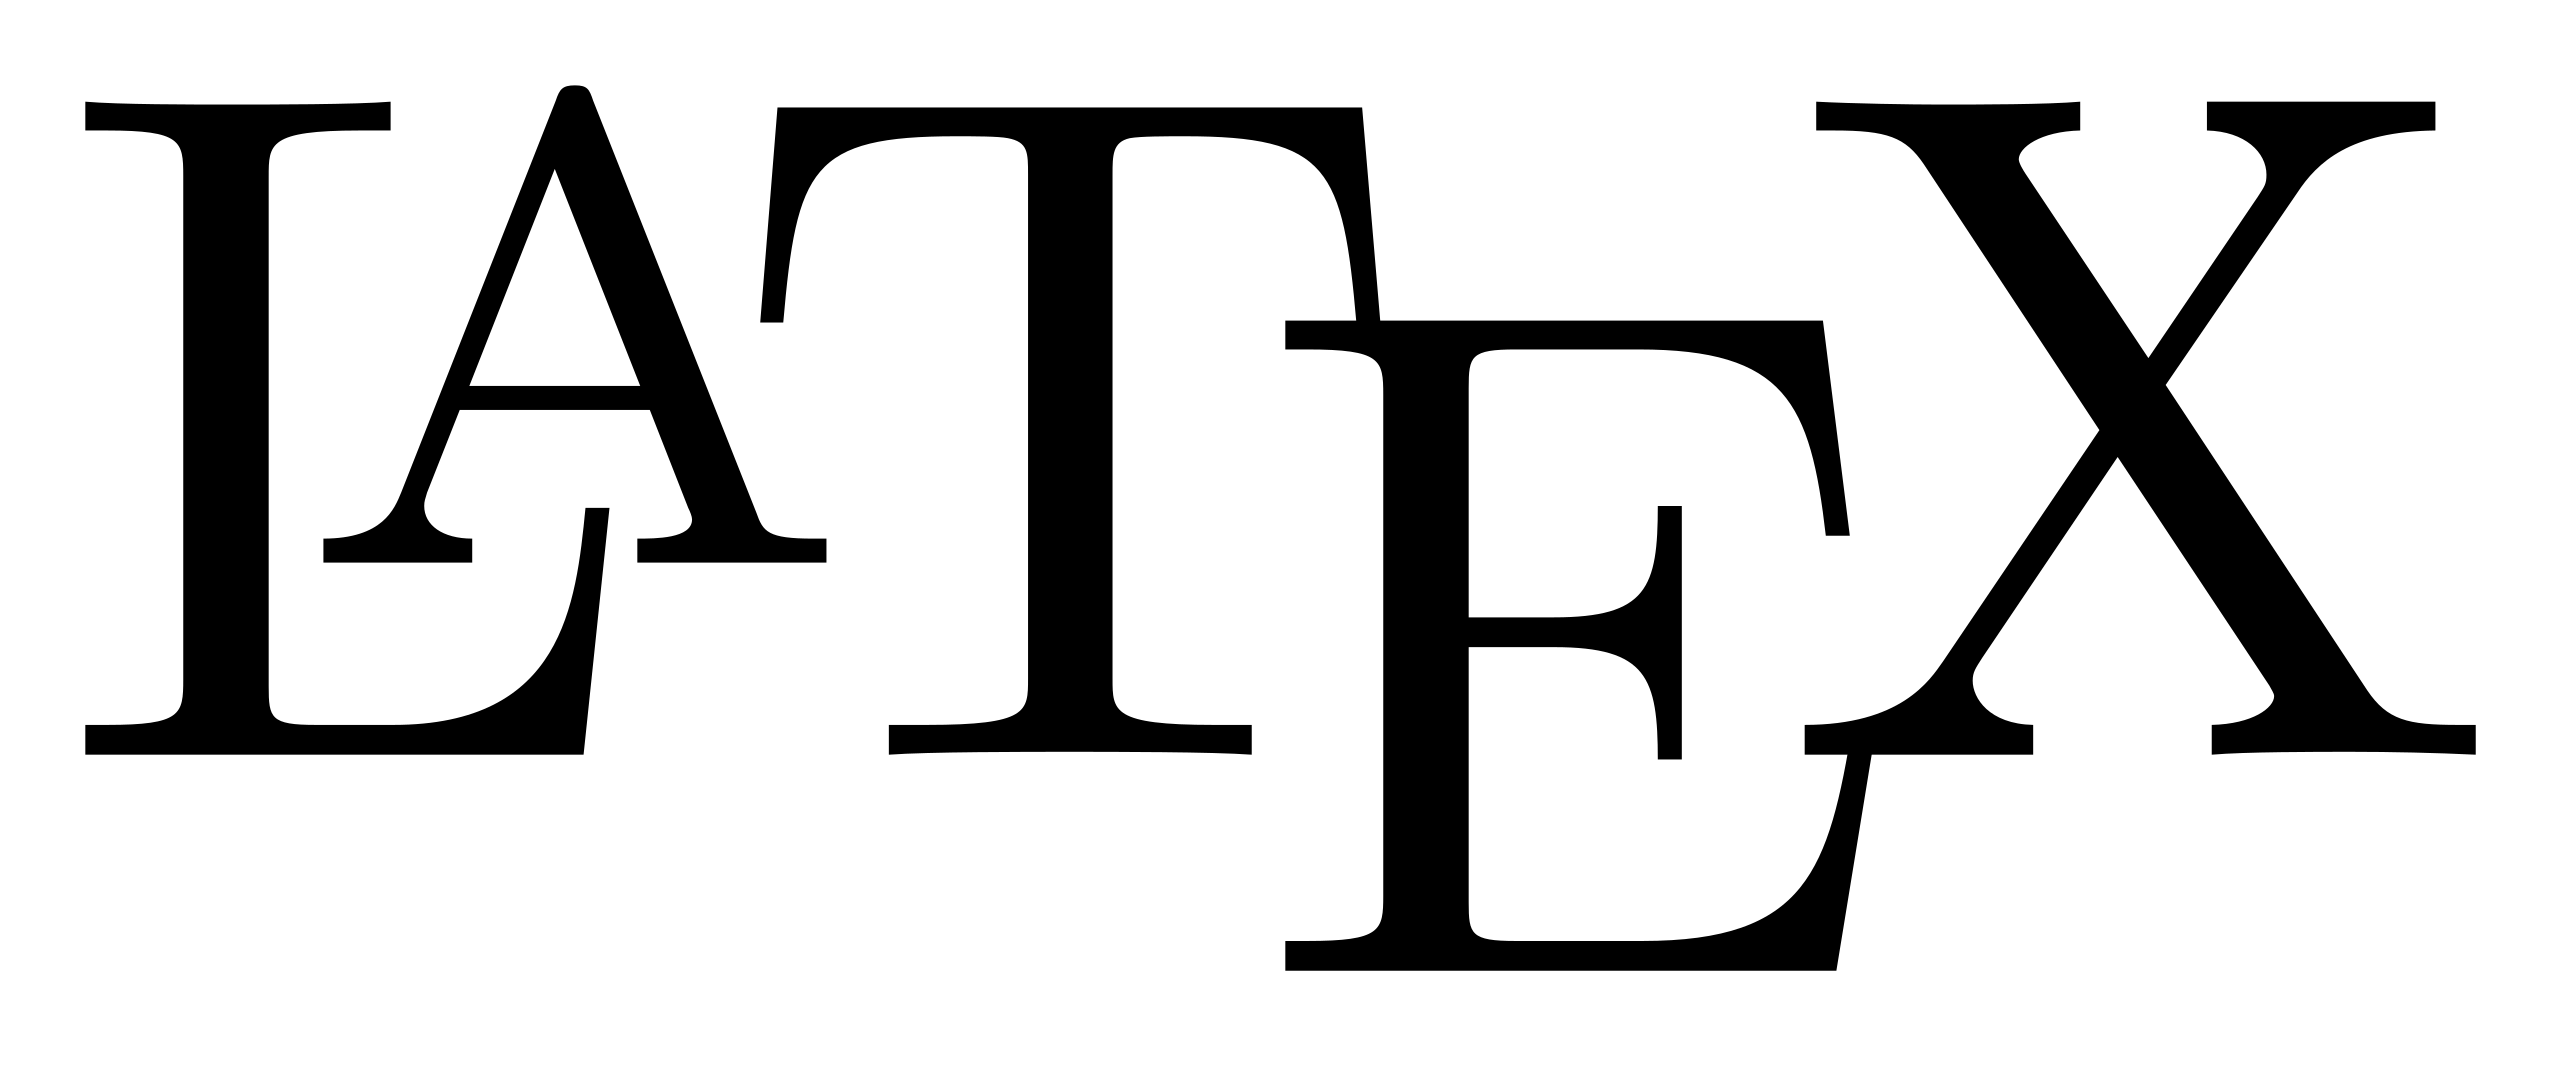
\includegraphics[width=0.10\textwidth]{images/latex}
        \vspace{-50pt}
    \end{wrapfigure} \noindent
    \textbf{LaTeX: }  An API platform for developers used to test your API endpoints,  we used it test our node.js API and asp.net API.

    \clearpage

    \begin{wrapfigure}{R}{0.10\textwidth}
        
\includegraphics[width=0.10\textwidth]{images/twillio}
        \vspace{-40pt}
    \end{wrapfigure} \noindent
    \textbf{Twilio: }   provides programmable communication tools for making and receiving phone calls, sending and receiving text messages, and performing other communication functions using its web service APIs.
    we used it to send sms message for Two factor authentication.

    \begin{wrapfigure}{R}{0.10\textwidth}
        
\includegraphics[width=0.10\textwidth]{images/vim}
        \vspace{-30pt}
    \end{wrapfigure} \noindent
    \textbf{Vim: }  Vim is a free and open-source, screen-based text editor program.
    It comes with Unix and it's known to be fast and powerful, because it can be managed entirely without menus or a mouse
    It is an improved clone of Bill Joy's vi. \\
    used to develop all the nodejs server.

    \noindent
    \textbf{Postman: }  A powerful software for designing user interfaces, we used it to create all the wire-frames.

    \noindent
    \textbf{Figma: }  A collaboration tool that organizes your projects into boards, We used it to track our progress on each chapter and assign tasks to members.

    \noindent
    \textbf{PlantUML: }  An open-source tool that allows you to create diagrams using a domain-specific language, we used it to create UML diagrams. 

     \textbf{Browser extensions }:
    \begin{itemize}
        \item  React Developer Tools: React Developer Tools is a Browser DevTools extension for the open-source React JavaScript library.
        It allows you to inspect the React component hierarchies in the Browser’s Developer Tools.
        \item Cookie editor (EditThisCookie):  A browser extension that allows you to edit your cookie preferences quickly and easily.
        It offers a simple interface, is fast, and lets you change your cookie settings very quickly.
        \item  JSONVue: Pretty prints any object of type json.
        Typically, when encountering a JSON document (content type "application/json"), the browser shows only plain text.
        The JSONView extension formats and highlights JSON documents, and allows the collapse of arrays and objects.

    \end{itemize}

    \clearpage
    \subsection{Hardware Used}

    \subsubsection{Laptop 1: }
    \underline{CPU} : AMD Ryzen 7 4800H with Radeon Graphics \\
    \underline{OS} :  Windows 10 \\
    \underline{RAM} :  16.0 GB \\
    \underline{Disk} :  500 GB SSD \\
    \underline{Graphic Card} : NVIDIA GeForce GTX 1660 Ti
    \subsubsection{Laptop 2: }
    \underline{CPU} :  intel i7-8565U @ 1.80GHz (8 CPUs) \\
    \underline{OS} :  Kali Linux os \\
    \underline{RAM} : 8 GB \\
    \underline{Disk} :  128 GB SSD + 1 TB HDD \\
    \underline{Graphic Card} :  Intel UHD Graphics 620
    \subsubsection{Laptop 3: }
    \underline{CPU} :  intel i7-8565U @ 1.80GHz (8 CPUs) \\
    \underline{OS} :  Windows 11 Pro 64-bit \\
    \underline{RAM} : 24.0 GB \\
    \underline{Disk} :  128 GB SSD + 1 TB HDD \\
    \underline{Graphic Card} :  Intel UHD Graphics 620 + AMD Radeon 520

    \section{Languages and Frameworks: }
     In this section we will list all the programming languages and frameworks that we used in our project, the motivation for their use and their importance in the security aspect of our system. \clearpage
    \noindent
    \textbf{JavaScript} :  one of the most popular scripting languages, know for it’s speed in performance, simplicity and modernity as it it can run in browsers, desktop and mobile apps, that’s exactly why we used it in the management part of our system to handle massive amounts of requests and data manipulation, display and validation in the fastest, modern and simplest way. \\

    \noindent
    \textbf{ReactJs} :  A free and open-source, most known front-end JavaScript library for building user interfaces based on UI components, there is a lot of advantages of using react we list:
    \begin{itemize}
        \item Reusability: react makes it very easy to create and use components, this is the advantage of using react.
        Tables, forms,calendar, menus are one component but they are used in different pages to display different information.
        \item state and hooks:  introduced in the React 16.8 version, “Hooks are functions that let you “hook into” React state and lifecycle features from function components.
        Hooks don’t work inside classes — they let you use React without classes”, in other words, react separates data from the UI and the components, this advantage give us the ability to use the same data in multiple places without duplicating that data and creating multiple copies (one single source of truth).
        \item Virtual DOM:  React uses Virtual DOM which is like a lightweight copy of the actual DOM (a virtual representation of the DOM).
        So for every object that exists in the original DOM, there is an object for that in React Virtual DOM. It is exactly the same, but it does not have the power to directly change the layout of the document.
        Manipulating DOM is slow, but manipulating Virtual DOM is fast as nothing gets drawn on the screen.
        \item Single page application: In a website done entirely in HTML, when clicking on links and if those links are internal, the url in the browser will be updated to the location of another page on the site (if the link is external, the user leaves the service).
        \item But the typical architecture of a react app is a “single page application”, meaning there is only one single “shell” HTML file, the content and interaction coming from javascript and data.
    \end{itemize}
    \textbf{Nodejs} : An open-source, cross-platform, back-end JavaScript runtime environment that runs on the V8 engine and executes JavaScript code outside a web browser.
    chose nodejs because of its advantage of handling many requests in very fast way, as long they are not heavy calculations. \\

    \noindent
    \textbf{Expressjs: } A backend web framework for Node.js.
    designed for building web applications and APIs.
    helps writing the nodejs server faster. \\

    \noindent
    \textbf{C\#: } A general-purpose object-oriented programming language made by Microsoft in 2000, it’s used to develop web apps, desktop apps, mobile apps, games and much more.
    The motivation to use C\#  was because it has a wide range of usages so we can use it in many parts of our system.
    we used it to develop the desktop client app and it's ASP.NET server. \\

    \noindent
    \textbf{Xaml: } A declarative XML-based language developed by Microsoft used exclusively to create user interfaces for .NET applications.
    used to build the desktop client user interfaces.\\

    \noindent
    \textbf{Avalonia: } An open source cross-platform UI framework, providing a flexible styling system and supporting a wide range of Operating Systems such as Windows, Linux, and MacOS using C# and .NET.
    we chose Avalonia because it’s the most stable and supported desktop cross-platform framework out there, for example we could have used the new .NET MAUI that’s made by Microsoft but we did’t because it’s not stable and has many bugs yet to be fixed.\\

    \noindent
    \textbf{ASP.NET: }  An open source cross-platform framework made by Microsoft to create Web applications and Web APIs using C# and .NET. We chose ASP.NET because it’s the same Back-end API used in similar secure online exam systems systems, and because it fits well in the .NET ecosystem. \\

    \subsubsection{Packages and libraries: }
      all of the Packages and libraries used on this project are listed on the appendix.

    \section{Security}

    \hspace*{8mm}  According to the HackerOneReport of the year 2019,  client-side vulnerabilities  make around 45\%  of total cyber-security  vulnerabilities,  with that in mind we tried to make our  client applications as secure as possible.
    For the web client, React helps prevent most Cross-Site Scripting (XSS) vulnerabilities due to how it creates DOM nodes and textual content.
    In any case, user input should have HTML entities escaped. \\
    \parindent  As for desktop client application it has the following features:
    \begin{itemize}
        \item Client-side input validation to reject any suspicions characters  and prevent any injections.
        \item Used the MVVM design-pattern to ensure the separation of the program logic and user interfaces as much as possible.
        \item Obfuscating the source code before building the executable application to make it extremely difficult to understand and modify the source code if someone did reverse-engineered the executable file , because Obfuscation makes the source code unreadable but keeps it fully functional.

        \begin{figure}[h]
            \centering
            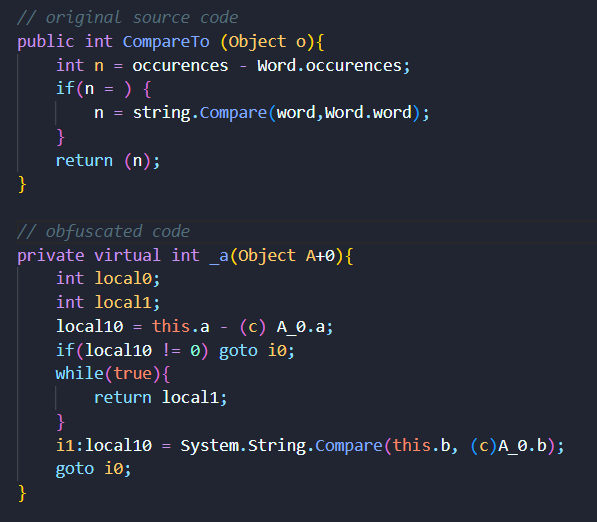
\includegraphics[width=250pt]{images/obs}
            \caption{Original source code VS Obfuscated source code}
        \end{figure}

        \item We also implemented some additional features to prevent Students from cheating:
        \begin{itemize}
            \item The application is always maximized,  TopMost (always on top) and can’t be re-sized.
            \item Used the windows native Api to block the program window from being recorded or screenshotted by any external software to prevent the student from sharing his screen while examining.
            \item We made a list of prohibited programs that are not allowed to run when the student is taking the exam like web browsers, in order to block such programs we scan the running processes on the student machine every 5 seconds and kill any process that exists in that list.
            \item When the application is opened it scans for connected monitors and warns the student if has more then one monitor connected , when the exam  starts if the program detects any external monitor the student will be kicked.
            \item The application registers internet cuts and it's durations, if a student’s internet connection cuts for a long time (more than 5 seconds) or cuts more than once he will be kicked.
        \end{itemize}
    \end{itemize}

    \hspace*{8mm} As for the backend, in addition of client-side input validation, we have server-side data validation as well, we also configured private routes for each role in our system, with this implementation each user is limited only to what he is supposed to see in addition to the api security where data is sent based on the authenticated user role. \\
    \hspace*{8mm} Lastly, For the database, we don't store plain passwords, instead they are encrypted before storing.



    \section{Conclusion}
    \hspace*{8mm}
\end{document}